\begin{figure}[p]
\centering
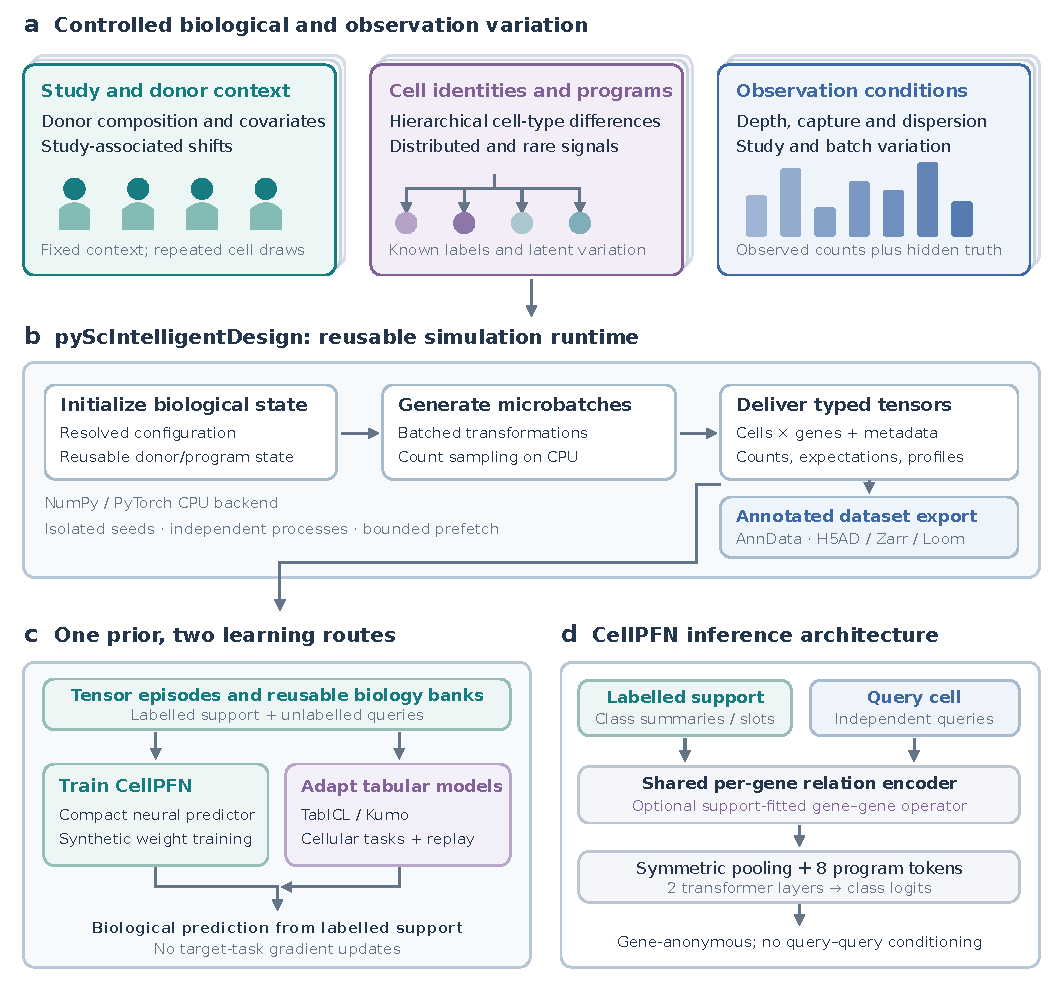
\includegraphics[width=\textwidth]{figures/architecture.pdf}
\caption{\textbf{A reusable cellular simulator supplies two learning routes.}
\textbf{a,} Configurable donor context, cell identities and expression programs are combined with observation conditions to generate cells with known labels and latent truth.
\textbf{b,} pyScIntelligentDesign separates initialization of biological state from repeated microbatch generation. CPU computation combines NumPy and PyTorch; typed tensors connect generation to training, while annotated exports support independent dataset use. Independent producer processes and bounded prefetch overlap task generation with training. Hidden profiles and expectations support diagnostics and are excluded from classifier inputs.
\textbf{c,} Tensor episodes and reusable biology banks train compact CellPFN or continue training released tabular models with cellular tasks and generic replay. Both applications perform downstream inference from labelled support without target-task gradient updates.
\textbf{d,} CellPFN compares each query with support-derived gene summaries and learned slots, optionally incorporating a support-fitted gene--gene operator. Symmetric aggregation and learned program tokens feed a transformer and class prediction head. The tokens are computational summaries, not annotated biological pathways. The schematic describes architecture and data flow; shapes do not represent measured quantities.}
\label{fig:architecture}
\end{figure}
